\documentclass[10pt]{article}
\usepackage[utf8]{inputenc}
\usepackage[T1]{fontenc}
\usepackage{lmodern}
\usepackage[letterpaper,top=1.18cm,bottom=1.15cm,left=1.28cm,right=1.28cm]{geometry}
\usepackage{graphicx,booktabs,amsmath,hyperref,array,tabularx,multicol}
\usepackage{xcolor}

\definecolor{navy}{HTML}{102A43}
\definecolor{blue}{HTML}{184E77}
\definecolor{teal}{HTML}{2A9D8F}
\definecolor{mint}{HTML}{DDF4EF}
\definecolor{pale}{HTML}{EDF5FB}
\definecolor{gold}{HTML}{D79B24}
\definecolor{sand}{HTML}{FFF4D6}
\definecolor{red}{HTML}{C95745}
\definecolor{rose}{HTML}{FCEAE6}
\definecolor{ink}{HTML}{172033}
\definecolor{muted}{HTML}{526B7A}
\definecolor{line}{HTML}{C9D9E6}

\hypersetup{colorlinks=true,urlcolor=blue,linkcolor=blue,pageanchor=false}
\setlength{\parindent}{0pt}
\setlength{\parskip}{3.2pt}
\setlength{\tabcolsep}{4.2pt}
\renewcommand{\arraystretch}{1.14}
\pagestyle{plain}
\newcolumntype{Y}{>{\raggedright\arraybackslash}X}
\newcolumntype{R}{>{\raggedleft\arraybackslash}X}

\newcommand{\pagetitle}[2]{%
  {\color{navy}\LARGE\bfseries #1\par}
  \vspace{1.5pt}{\color{teal}\rule{\linewidth}{1.6pt}}\vspace{2pt}
  {\color{muted}\small #2\par}\vspace{5pt}
}
\newcommand{\takeaway}[1]{%
  \begingroup\setlength{\fboxsep}{7pt}%
  \noindent\colorbox{mint}{\parbox{\dimexpr\linewidth-2\fboxsep\relax}{\color{navy}\small\textbf{Conclusión.} #1}}%
  \endgroup
}
\newcommand{\warningbox}[1]{%
  \begingroup\setlength{\fboxsep}{6pt}%
  \noindent\colorbox{sand}{\parbox{\dimexpr\linewidth-2\fboxsep\relax}{\color{ink}\small #1}}%
  \endgroup
}
\newcommand{\metricbox}[3]{%
  \begingroup\setlength{\fboxsep}{5pt}%
  \colorbox{pale}{\parbox[c][1.13cm][c]{#1}{\centering{\color{teal}\Large\bfseries #2}\par\vspace{1pt}{\color{muted}\scriptsize\bfseries #3}}}%
  \endgroup
}
\newcommand{\subhead}[1]{\vspace{2pt}{\color{blue}\bfseries #1}\par\vspace{1pt}}

\begin{document}

% PÁGINA 1 — PORTADA EJECUTIVA
\begin{titlepage}
\pagecolor{navy}\color{white}
\vspace*{0.35cm}
{\small\bfseries DEEP LEARNING Y SISTEMAS INTELIGENTES \hfill PROYECTO 1 · V5 FINAL\par}
\vspace{0.35cm}{\color{teal}\rule{\linewidth}{2pt}}
\vspace{0.75cm}
{\Huge\bfseries Monitoreo transaccional\par}
\vspace{0.18cm}{\LARGE Detectar lo que el orden revela\par}
\vspace{0.8cm}

\begingroup\setlength{\fboxsep}{10pt}
\colorbox{blue}{\parbox{\dimexpr\linewidth-2\fboxsep\relax}{%
  {\large\bfseries Pregunta ejecutiva}\par\vspace{3pt}
  ¿Incorporar una GRU mejora la priorización de fraude frente a un modelo tabular competitivo y justifica su costo operativo?
}}
\endgroup

\vspace{0.75cm}
\begin{tabularx}{\linewidth}{@{}XXXX@{}}
\metricbox{0.88\linewidth}{590,540}{transacciones reales}&
\metricbox{0.88\linewidth}{3.50\%}{prevalencia de fraude}&
\metricbox{0.88\linewidth}{0.545}{AP del candidato A}&
\metricbox{0.88\linewidth}{0.908}{ROC--AUC de A}
\end{tabularx}

\vspace{0.72cm}
\begingroup\setlength{\fboxsep}{11pt}
\colorbox{teal}{\parbox{\dimexpr\linewidth-2\fboxsep\relax}{%
  {\Large\bfseries Decisión: conservar A}\par\vspace{4pt}
  LightGBM ofrece el mejor ranking operativo y el menor costo. B recupera algunos fraudes adicionales, pero multiplica las falsas alarmas; permutar su historia no reduce AP. C tampoco alcanza el criterio previo de éxito. La evidencia no justifica migrar a un modelo secuencial.
}}
\endgroup

\vfill
\begin{tabularx}{\linewidth}{@{}Y Y@{}}
\textbf{Universidad del Valle de Guatemala}\newline
Facultad de Ingeniería · Sección 30\newline
Docente: Kevin Recinos\newline
Semestre II · 2026
&
\textbf{Equipo}\newline
Wilson Alejandro Calderón Argueta · 22018\newline
Pablo Daniel Barillas Moreno · 22193\newline
Modalidad: parejas
\end{tabularx}
\vspace{0.3cm}
\end{titlepage}
\hypersetup{pageanchor=true}
\setcounter{page}{1}
\nopagecolor\color{ink}

% PÁGINA 2 — RESUMEN Y PROTOCOLO
\pagetitle{1 · Resumen ejecutivo y protocolo temporal}{La comparación es válida solo si A, B y C ven las mismas observaciones y ninguna transformación aprende del futuro.}

\takeaway{A es el candidato porque maximiza AP interno y minimiza costo. La pregunta central también queda respondida: con esta identidad proxy, estas variables y esta arquitectura, el orden no aporta evidencia predictiva material.}

\vspace{5pt}
\begin{minipage}[t]{0.49\linewidth}
\subhead{Diseño de la investigación}
\normalsize
\textbf{A · Sin orden.} LightGBM con expertos por \texttt{ProductCD}, variables actuales y agregados históricos causales. Establece cuánto puede lograrse sin leer la secuencia.\par
\textbf{B · Secuencial.} GRU causal que recibe la transacción objetivo y hasta 15 antecedentes ordenados. Pregunta si el orden agrega señal.\par
\textbf{C · Apuesta.} Stacking logístico de los puntajes A/B, monto, longitud de historia y producto. Se declaró útil solo con $\Delta AP\ge 0.01$ y reducción de costo $\ge5\%$.

\subhead{Qué se predice}
Cada fila recibe un puntaje continuo de riesgo para la transacción actual. El umbral se selecciona después y no modifica la calidad del ranking medida por AP o ROC--AUC.
\end{minipage}\hfill
\begin{minipage}[t]{0.48\linewidth}
\subhead{Integridad de datos}
\normalsize
\textbf{Origen:} IEEE--CIS Fraud Detection, 590,540 filas y 20,663 fraudes. Las tablas se unen por \texttt{TransactionID} y se ordenan por \texttt{TransactionDT}; ambos campos se excluyen como magnitudes predictivas.\par
\textbf{Entidad:} \texttt{card1+card2+card3+card5+addr1}. Es una aproximación de tarjeta/cliente, no una identidad bancaria.\par
\textbf{Secuencia:} objetivo más hasta 15 antecedentes; 76.3\% de las filas tiene al menos 8 eventos y 66.2\% llega a 16.\par
\textbf{Causalidad:} toda variable histórica satisface
\[
x_t^{hist}=f\!\left(\{x_j:t_j<t\}\right).
\]
Imputación, categorías, escalado, calibración y umbrales se ajustan antes del bloque evaluado.
\end{minipage}

\vspace{5pt}
\subhead{Partición cronológica y función de cada bloque}
\begin{tabularx}{\linewidth}{@{}p{2.15cm}p{2.25cm}Y Y@{}}
\toprule
\textbf{Período} & \textbf{Filas} & \textbf{Uso permitido} & \textbf{Control contra fuga}\\
\midrule
Entrenamiento 70\% & 413,378 & Ajustar A/B y preprocesamiento & Solo observaciones antiguas\\
Validación 15\% & 88,581 & Early stopping, meta-modelo, calibración, umbral y evaluación interna en bloques separados & Cada decisión precede al bloque donde se mide\\
Benchmark 15\% & 88,581 & Referencia temporal histórica & No se usa para seleccionar V5; ya no se presenta como test ciego\\
\bottomrule
\end{tabularx}

\vspace{5pt}
\begin{minipage}[c]{0.62\linewidth}
\centering
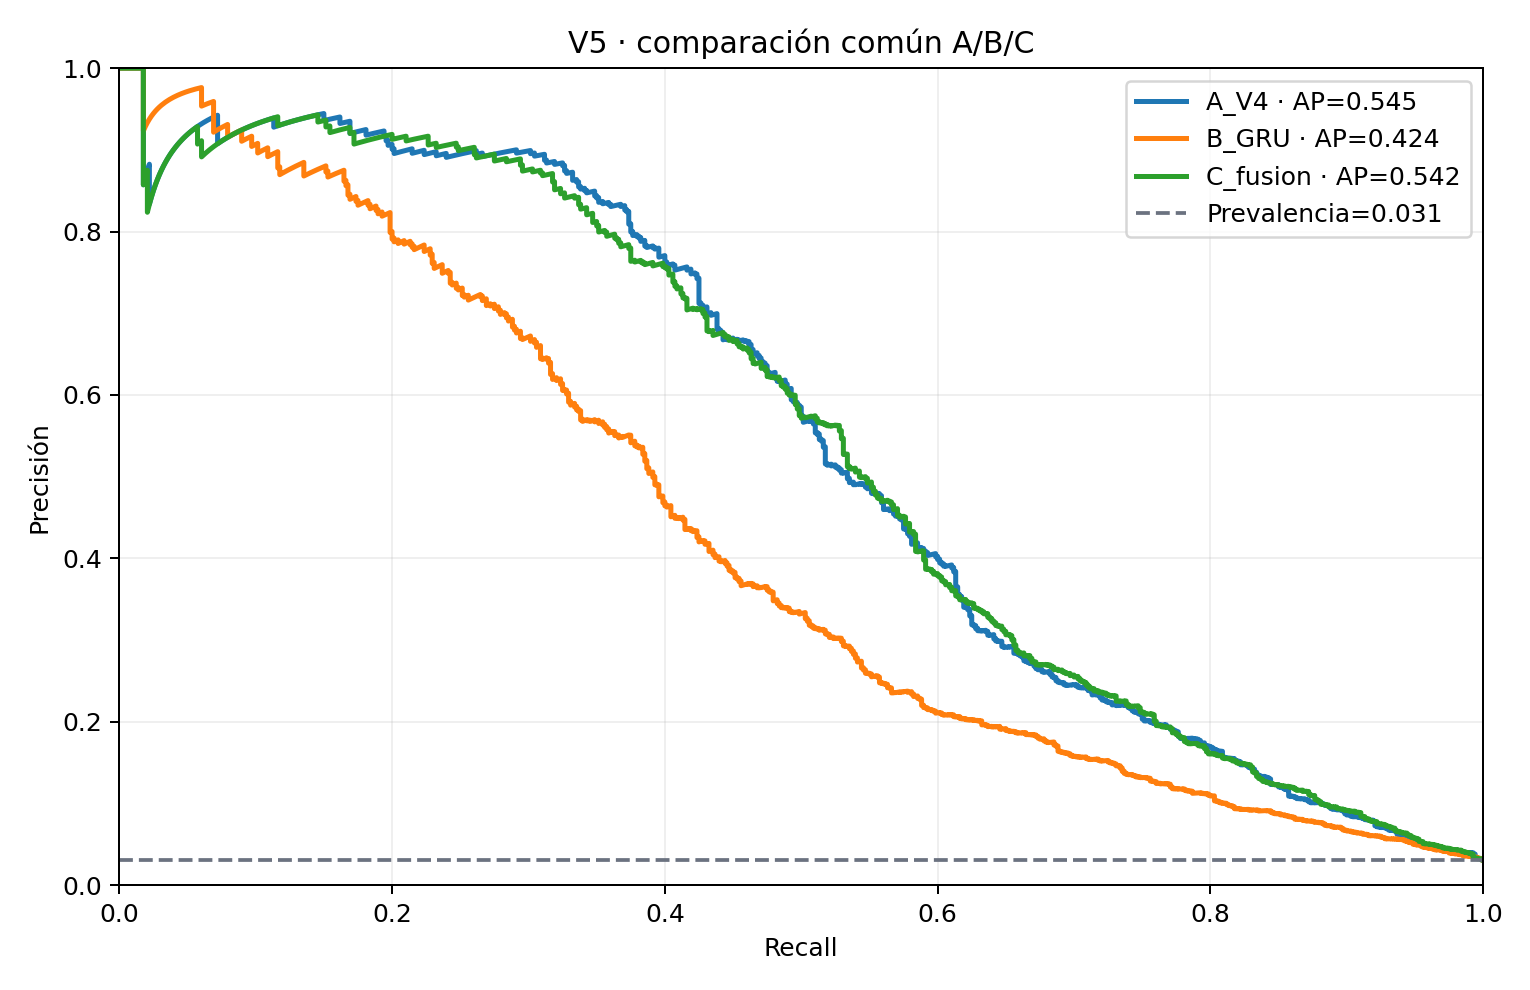
\includegraphics[width=\linewidth]{../../../evidencia/figuras/v5/01_comparacion_abc_validacion.png}
\end{minipage}\hfill
\begin{minipage}[c]{0.35\linewidth}
\normalsize
\textbf{Lectura de la curva PR}\par
La prevalencia interna es 3.07\%, por lo que un ranking aleatorio tendría AP cercano a 0.031. A alcanza 0.545: aproximadamente 17.7 veces esa referencia. C casi lo iguala; B queda claramente por debajo.\par
\vspace{3pt}
\textbf{Resultado que debe recordarse}\par
La señal tabular es fuerte. La señal secuencial, bajo el diseño probado, no es complementaria ni estable.
\end{minipage}

\vfill
\warningbox{\textbf{Alcance de validez.} El 15\% final se conserva como benchmark histórico porque ya fue observado durante la evolución V1--V5. Las decisiones de V5 se toman dentro de bloques cronológicos de validación; una afirmación confirmatoria requiere una cohorte etiquetada nueva.}

\clearpage

% PÁGINA 3 — COMPARACIÓN
\pagetitle{2 · Comparación común A/B/C}{Núcleo A/B y apuesta C: AP y ROC--AUC evalúan ranking; precisión, recall, F1 y costo describen el umbral operativo.}

\begin{tabularx}{\linewidth}{@{}p{1.2cm}Y Y Y@{}}
\toprule
\textbf{Modelo} & \textbf{Representación} & \textbf{Fortaleza esperada} & \textbf{Control experimental}\\
\midrule
\textbf{A} & LightGBM, expertos W/NO--W y agregados causales & Interacciones no lineales en datos tabulares & No recibe eventos ordenados\\
\textbf{B} & 57 numéricas, 12 categóricas con embeddings, proyección 96 y GRU(64) & Dependencias entre antecedentes & Misma población, horizonte y objetivo que A\\
\textbf{C} & Regresión logística sobre logits A/B, monto, historia y producto & Complementariedad de errores & Meta-ajuste y evaluación en bloques posteriores separados\\
\bottomrule
\end{tabularx}

\vspace{5pt}
\subhead{Resultado principal en evaluación interna temporal}
\begin{center}
\begin{tabular}{lrrrrrrrr}
\toprule
\textbf{Modelo}&\textbf{AP}&\textbf{ROC}&\textbf{Prec.}&\textbf{Recall}&\textbf{F1}&\textbf{Costo}&\textbf{Alertas/100k}\\
\midrule
\textbf{A}&\textbf{0.545}&0.908&\textbf{0.220}&0.738&\textbf{0.339}&\textbf{Q1,067,460}&\textbf{10,291}\\
B&0.424&0.877&0.132&0.749&0.224&Q1,320,840&17,416\\
C&0.542&\textbf{0.911}&0.173&\textbf{0.785}&0.284&Q1,072,020&13,921\\
\bottomrule
\end{tabular}
\end{center}

\begin{minipage}[t]{0.49\linewidth}
\subhead{Qué dicen AP y ROC}
\normalsize
\textbf{AP 0.545} no significa 54.5\% de precisión en el umbral. Resume la precisión obtenida a medida que cambia el recall. A concentra fraudes en la parte alta del ranking y supera a B por 0.120 AP.\par
\textbf{ROC 0.908} indica buena separación global, pero puede ocultar carga operativa: una tasa moderada de falsos positivos aplicada a 96.9\% de negativos produce miles de alertas. Por eso AP es la métrica principal.

\subhead{Estabilidad temporal}
A pasa de AP 0.545 interno a 0.559 en benchmark, y de ROC 0.908 a 0.901. La variación es pequeña y respalda que el ranking tabular es relativamente estable.
\end{minipage}\hfill
\begin{minipage}[t]{0.48\linewidth}
\subhead{Qué dice la matriz de confusión}
\normalsize
\begin{tabularx}{\linewidth}{@{}lrrrr@{}}
\toprule
&\textbf{TP}&\textbf{FP}&\textbf{FN}&\textbf{Alertas falsas}\\
\midrule
A&502&1,777&178&78.0\%\\
B&509&3,348&171&86.8\%\\
C&534&2,549&146&82.7\%\\
\bottomrule
\end{tabularx}
\vspace{4pt}
A detecta 73.8\% de los fraudes, pero 1,777 de sus 2,279 alertas son legítimas. B encuentra solo siete fraudes adicionales y genera 1,571 falsas alarmas más. C encuentra 32 adicionales y agrega 772 falsas alarmas.

\subhead{Por qué F1 no decide solo}
F1 pondera precisión y recall por igual; el escenario económico no. Un falso negativo cuesta 23.3 veces un falso positivo, de modo que el umbral favorece recall aun cuando reduzca F1.
\end{minipage}

\vspace{6pt}
\warningbox{\textbf{Veredicto de C: no útil.} Frente al mejor individual, C cambia AP en $-0.0020$ y el costo en $-0.43\%$ de ``reducción''; no alcanza ni $+0.01$ AP ni $5\%$ de ahorro. El pequeño aumento de recall no compensa su volumen de falsas alarmas.}

\vspace{5pt}
\begin{tabularx}{\linewidth}{@{}XXX@{}}
\metricbox{0.90\linewidth}{17.7$\times$}{AP de A frente al azar}&
\metricbox{0.90\linewidth}{7.17$\times$}{precisión frente a prevalencia}&
\metricbox{0.90\linewidth}{8.28\%}{legítimas marcadas por A}
\end{tabularx}

\vfill
\takeaway{A gana por la combinación que importa: mejor AP, mejor F1 operativo y menor costo. B y C no son modelos absurdos; simplemente compran recall a un precio de falsas alarmas que el escenario económico no justifica.}

\clearpage

% PÁGINA 4 — ORDEN
\pagetitle{3 · ¿El orden aporta información?}{Una métrica alta de B no demostraría uso del orden; por eso se intentó refutar la hipótesis mediante dos falsificaciones.}

\begin{minipage}[c]{0.65\linewidth}
\centering
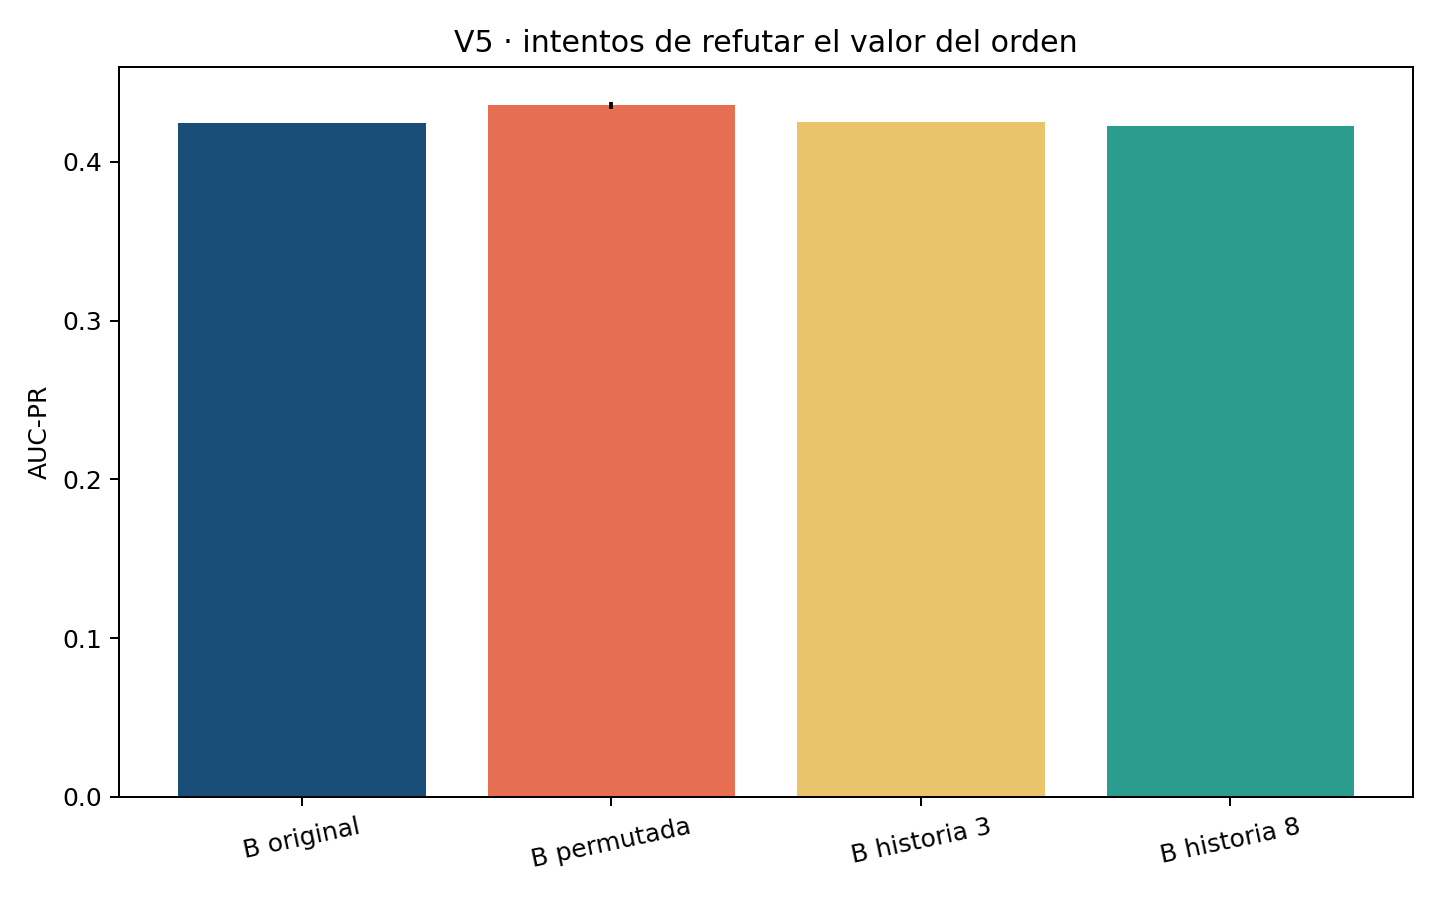
\includegraphics[width=\linewidth]{../../../evidencia/figuras/v5/03_falsificaciones_orden_v5.png}
\end{minipage}\hfill
\begin{minipage}[c]{0.32\linewidth}
\normalsize
\begin{tabularx}{\linewidth}{@{}Y R@{}}
\toprule
\textbf{Condición} & \textbf{AP}\\
\midrule
B original & 0.4245\\
Historia permutada & $0.4355\pm0.0021$\\
Historia de 3 & 0.4253\\
Historia de 8 & 0.4225\\
\bottomrule
\end{tabularx}
\vspace{5pt}
\textbf{Cambio por permutación:}
\[
0.4245-0.4355=-0.0111.
\]
El signo es contrario al esperado si el orden fuera útil.
\end{minipage}

\vspace{5pt}
\begin{minipage}[t]{0.49\linewidth}
\subhead{Prueba 1 · Permutación controlada}
\normalsize
Se barajan únicamente los antecedentes dentro de cada secuencia. Se conservan eventos, valores, longitud, variables agregadas y transacción objetivo. La prueba se repite con cinco semillas.\par
\textbf{Predicción falsable:} si B usa el orden, AP debería disminuir de forma consistente.\par
\textbf{Observación:} AP aumenta en las cinco permutaciones. La variación entre semillas es pequeña frente a la diferencia observada. No hay evidencia de dependencia útil del orden.
\end{minipage}\hfill
\begin{minipage}[t]{0.48\linewidth}
\subhead{Prueba 2 · Recorte de historia}
\normalsize
Se evalúa el mismo B con ventanas de 3 y 8 eventos, frente a la historia máxima de 16.\par
\textbf{Predicción falsable:} si antecedentes lejanos aportan memoria, reducir la ventana debería deteriorar AP.\par
\textbf{Observación:} 3 eventos producen 0.4253, prácticamente igual al original; 8 produce 0.4225. La longitud adicional no entrega una ganancia material.
\end{minipage}

\vspace{5pt}
\subhead{La GRU también pierde calidad donde más importa}
\begin{tabularx}{\linewidth}{@{}p{2.2cm}RRR Y@{}}
\toprule
\textbf{Período} & \textbf{ROC} & \textbf{AP} & \textbf{Recall} & \textbf{Interpretación}\\
\midrule
Interno temporal & 0.877 & 0.424 & 0.749 & Ranking moderado con 86.8\% de alertas falsas\\
Benchmark histórico & 0.866 & 0.218 & 0.791 & ROC baja poco, pero el ranking superior de fraudes se degrada con fuerza\\
\bottomrule
\end{tabularx}

\vspace{4pt}
\textbf{Consistencia entre semillas.} Las cinco permutaciones obtienen AP 0.4331, 0.4371, 0.4386, 0.4355 y 0.4335: todas superan el 0.4245 original. El veredicto no depende de una única mezcla aleatoria.

\vspace{5pt}
\warningbox{\textbf{Qué no puede concluirse.} El experimento no demuestra que ``las GRU no sirven'' ni que ningún fraude dependa del orden. Solo demuestra que esta GRU, alimentada por esta clave proxy y este conjunto de variables, no extrae valor temporal adicional.}

\vfill
\takeaway{La respuesta principal del proyecto es negativa y concluyente dentro de su alcance: destruir el orden no perjudica a B y acortar la historia tampoco. Antes de aumentar capas o épocas debe mejorarse la identidad transaccional y demostrarse una caída real bajo permutación.}

\clearpage

% PÁGINA 5 — ECONOMÍA
\pagetitle{4 · Umbral, falsas alarmas y valor económico}{El umbral no intenta maximizar F1: minimiza costo bajo una restricción de recall aprendida en un bloque anterior.}

\begin{minipage}[c]{0.53\linewidth}
\centering
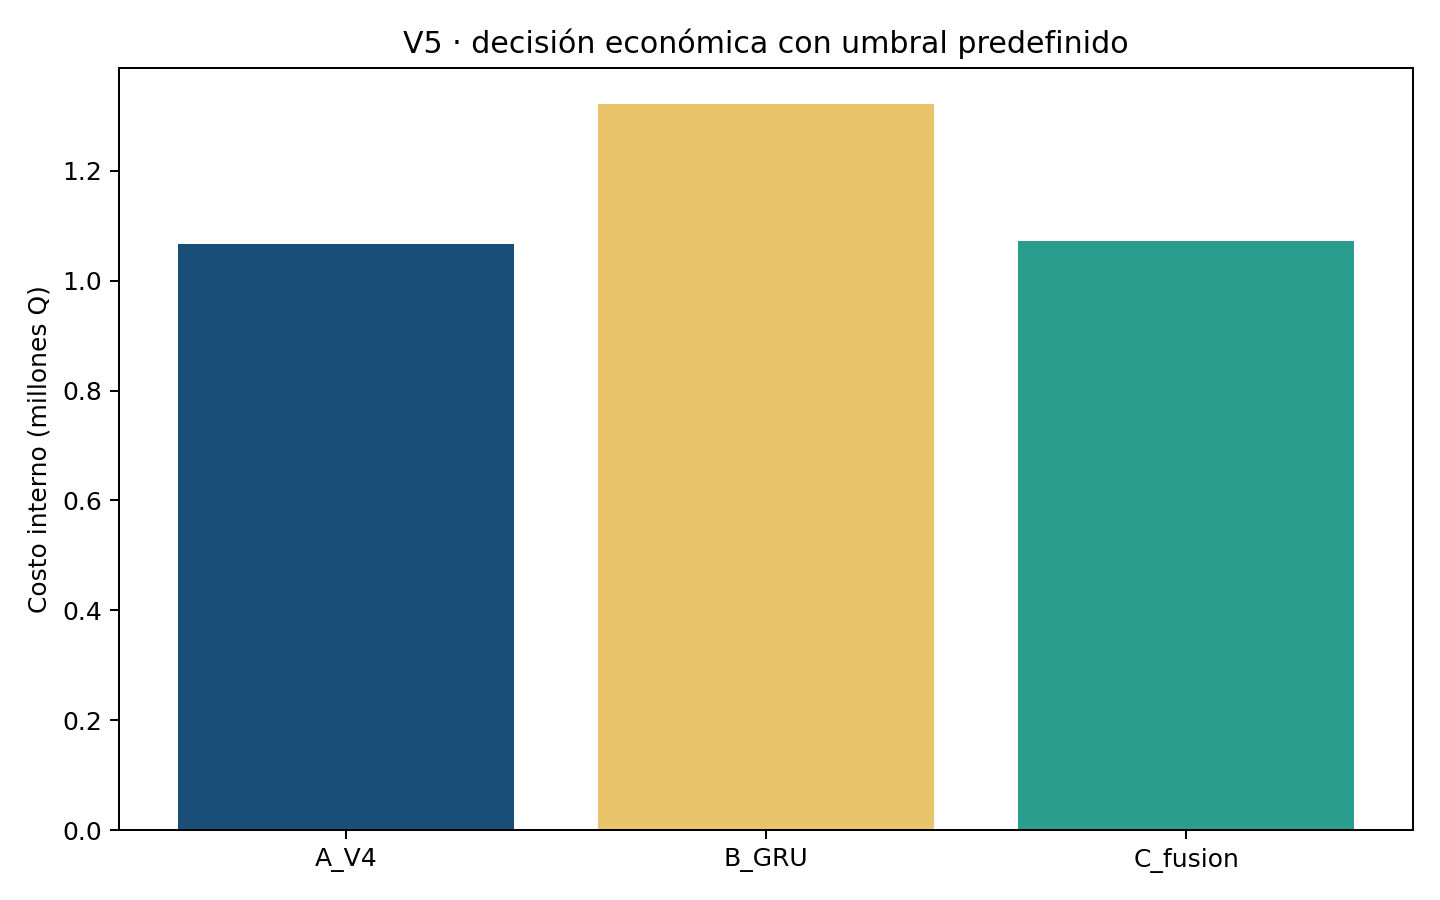
\includegraphics[width=\linewidth]{../../../evidencia/figuras/v5/04_costos_abc_v5.png}
\end{minipage}\hfill
\begin{minipage}[c]{0.44\linewidth}
\normalsize
\subhead{Política predefinida}
\[
C(\tau)=4200FN(\tau)+180FP(\tau),
\qquad Recall\ge0.75.
\]
Un fraude omitido cuesta lo mismo que 23.3 falsas alarmas. El umbral de A, $\tau=0.05783$, se fijó antes de la evaluación interna. Que su recall posterior sea 0.738 refleja deriva entre bloques, no reajuste sobre evaluación.

\begin{tabularx}{\linewidth}{@{}lRR@{}}
\toprule
\textbf{Modelo}&\textbf{Costo interno}&\textbf{Costo/decisión}\\
\midrule
A&Q1,067,460&Q48.20\\
B&Q1,320,840&Q59.64\\
C&Q1,072,020&Q48.41\\
\bottomrule
\end{tabularx}
\end{minipage}

\vspace{5pt}
\subhead{La diferencia de costo se explica completamente por los errores}
\begin{minipage}[t]{0.49\linewidth}
\normalsize
\textbf{B frente a A}\par
B evita 7 falsos negativos:
\[
7\times Q4{,}200=Q29{,}400.
\]
Pero agrega 1,571 falsos positivos:
\[
1{,}571\times Q180=Q282{,}780.
\]
El saldo es \textbf{Q253,380 peor}, exactamente la diferencia observada. Siete fraudes adicionales no justifican duplicar casi la carga de alertas.
\end{minipage}\hfill
\begin{minipage}[t]{0.48\linewidth}
\normalsize
\textbf{C frente a A}\par
C evita 32 falsos negativos:
\[
32\times Q4{,}200=Q134{,}400.
\]
Pero agrega 772 falsos positivos:
\[
772\times Q180=Q138{,}960.
\]
El saldo es \textbf{Q4,560 peor}. C queda cerca de A, pero no produce ahorro ni cumple la hipótesis previa.
\end{minipage}

\vspace{5pt}
\subhead{Qué recibiría un equipo de revisión por cada 100,000 transacciones}
\begin{tabularx}{\linewidth}{@{}lrrrrY@{}}
\toprule
\textbf{Modelo}&\textbf{Alertas}&\textbf{Fraudes detectados}&\textbf{Falsas alarmas}&\textbf{Precisión}&\textbf{Lectura operativa}\\
\midrule
A&10,291&$\approx2,267$&$\approx8,024$&22.0\%&Mejor carga entre los tres, aún alta\\
B&17,416&$\approx2,299$&$\approx15,117$&13.2\%&Inviable sin mayor capacidad o filtro\\
C&13,921&$\approx2,411$&$\approx11,510$&17.3\%&Más recall, sin ventaja económica\\
\bottomrule
\end{tabularx}

\vspace{4pt}
\subhead{Escenario mensual central: 1.4 millones de tarjetas y 12 transacciones por tarjeta}
\begin{tabularx}{\linewidth}{@{}lRR Y@{}}
\toprule
\textbf{Modelo}&\textbf{Costo mensual proyectado}&\textbf{Diferencia frente a A}&\textbf{Lectura}\\
\midrule
A&Q927,422,359&Q0&Referencia de menor costo\\
B&Q1,092,992,854&Q165,570,495 peor&Mayor pérdida y carga\\
C&Q943,103,194&Q15,680,834 peor&Cercano, sin ahorro\\
\bottomrule
\end{tabularx}

\vspace{5pt}
\warningbox{\textbf{Interpretación correcta de la precisión.} Que 78\% de las alertas de A sean falsas no significa que el ranking sea inútil: AP 0.545 frente a una base aleatoria de 0.031 demuestra señal. Significa que el punto operativo compra recall con una carga humana considerable. Si el banco no puede revisar 10,291 alertas por 100,000 transacciones, debe definir un presupuesto de alertas y volver a seleccionar $\tau$ en una cohorte nueva.}

\vfill
\takeaway{A minimiza el costo académico, pero todavía no prueba viabilidad operativa. La promoción exige costos reales, capacidad diaria de revisión y métricas como Precision@K y Recall@K; no basta con una curva ROC alta.}

\clearpage

% PÁGINA 6 — RECOMENDACIÓN Y CONTEXTO
\pagetitle{5 · Recomendación, referencia externa y límites}{El resultado es defendible como investigación; no equivale a un sistema listo para producción.}

\begin{minipage}[t]{0.48\linewidth}
\subhead{Recomendación al comité de riesgos}
\normalsize
\textbf{Conservar A} como candidato para ordenar casos antes de la revisión humana. No reemplazarlo por B/C y no bloquear transacciones automáticamente. El puntaje indica prioridad, no culpabilidad.\par
\textbf{Patrón de error prioritario:} falsos negativos de monto alto. Se exportaron 100 casos para análisis; deben revisarse por producto, dispositivo, identidad disponible y novedad del comportamiento.\par
\textbf{Quién usa el puntaje:} analista de fraude. La salida es un riesgo continuo, el umbral vigente y una decisión de incluir o no la transacción en la cola de revisión.

\subhead{Cuándo cambiaría la decisión}
\begin{enumerate}
\item Una identidad bancaria fiable hace que permutar la historia reduzca AP de manera estable.
\item Una cohorte temporal nueva muestra que B/C reduce costo e intervalos de confianza excluyen cero.
\item La operación demuestra que puede absorber la carga de alertas sin afectar clientes legítimos.
\item Un ensamble tabular más fuerte supera a A bajo el mismo protocolo causal.
\end{enumerate}
\end{minipage}\hfill
\begin{minipage}[t]{0.49\linewidth}
\subhead{Contexto externo: útil, no directamente comparable}
\footnotesize
\begin{tabularx}{\linewidth}{@{}YRRR@{}}
\toprule
\textbf{Método IEEE--CIS}&\textbf{ROC}&\textbf{AP/AUPRC}&\textbf{F1}\\
\midrule
A V5, temporal interno&0.908&0.545&0.339\\
A V5, benchmark histórico&0.901&0.559&0.340\\
Kaggle 1.º, blend privado&0.945&--&--\\
Kaggle 17.º, ensemble privado&0.941&--&--\\
Han--Wu, LGBM aleatorio&0.934&0.648&0.609\\
Han--Wu, fusión aleatoria&0.941&0.670&0.637\\
\bottomrule
\end{tabularx}
\vspace{3pt}
Kaggle evaluó ROC--AUC y los equipos líderes combinaron identificación avanzada de clientes, ingeniería de variables, CatBoost, LightGBM y XGBoost. Han y Wu usan partición estratificada aleatoria; sus propios autores reconocen que no es temporal. Sus cifras son una referencia de potencial, no una comparación equivalente. A está por debajo del estado competitivo fuerte, pero conserva un protocolo más alineado con la rúbrica.

\subhead{Riesgos que impiden producción}
\footnotesize
\begin{tabularx}{\linewidth}{@{}p{2.15cm}Y@{}}
\toprule
\textbf{Riesgo}&\textbf{Implicación}\\
\midrule
Identidad proxy&Mezcla clientes o fragmenta una misma tarjeta\\
Benchmark reutilizado&No permite una afirmación confirmatoria nueva\\
Costos académicos&El umbral puede cambiar con pérdidas y capacidad reales\\
Deriva temporal&B pierde AP de 0.424 a 0.218\\
Anonimización&Limita explicación causal y diseño de controles\\
Gobernanza no evaluada&Faltan privacidad, equidad, seguridad, latencia, apelación y monitoreo\\
\bottomrule
\end{tabularx}
\end{minipage}

\vspace{4pt}
\subhead{Siguiente iteración con mayor probabilidad de mejorar}
\normalsize
\textbf{1.} Bloquear una cohorte temporal nueva. \textbf{2.} Mejorar UID e incorporar agregados causales por cliente/dispositivo. \textbf{3.} Comparar LightGBM, CatBoost y XGBoost con intervalos temporales. \textbf{4.} Seleccionar umbral por costo y capacidad de revisión. \textbf{5.} Reentrenar una secuencia solo si la permutación demuestra señal.

\vspace{4pt}
\begin{tabularx}{\linewidth}{@{}p{2.25cm}Y Y@{}}
\toprule
\textbf{Puerta de decisión}&\textbf{Evidencia exigida}&\textbf{Resultado actual}\\
\midrule
Pilotar A&Capacidad, costo real y revisión humana&Condicionado\\
Promover B/C&Menor costo y caída bajo permutación&No cumple\\
Bloqueo automático&Calibración, gobernanza y seguridad&No autorizado\\
\bottomrule
\end{tabularx}

\vspace{4pt}
\subhead{Referencias seleccionadas}
\footnotesize
Cho, K., et al. (2014). Learning phrase representations using RNN encoder--decoder. \textit{EMNLP}, 1724--1734.\quad
Han, X., \& Wu, C. (2026). Validation-stage combinatorial fusion analysis for imbalanced credit-card fraud detection. \textit{arXiv:2606.10393}.\quad
IEEE Computational Intelligence Society. (2019). \textit{IEEE--CIS Fraud Detection}. Kaggle.\quad
Ke, G., et al. (2017). LightGBM. \textit{NeurIPS, 30}.\quad
Saito, T., \& Rehmsmeier, M. (2015). The precision--recall plot is more informative than the ROC plot. \textit{PLOS ONE, 10}(3), e0118432.\quad
Yakovlev, K., \& Deotte, C. (2019). \textit{1st place solution, IEEE--CIS Fraud Detection}. Kaggle.

\vspace{4pt}
\takeaway{El modelo es un baseline académico fuerte y útil para priorización, no un sistema autónomo. Su principal mejora no es una GRU más grande: es mejor identidad, más señal causal, validación temporal nueva y un umbral ligado a capacidad real.}

\clearpage

% PÁGINA 7 — MATRIZ
\pagetitle{6 · Matriz de evidencias y veredicto final}{Guía compacta para localizar qué se probó, qué se concluye y hasta dónde llega cada afirmación.}

\footnotesize
\begin{tabularx}{\linewidth}{@{}p{2.05cm}p{2.15cm}Y Y@{}}
\toprule
\textbf{Evidencia} & \textbf{Ubicación} & \textbf{Resultado y conclusión} & \textbf{Limitación o condición}\\
\midrule
Integridad de datos & Sec. 1; Fig. PR & 590,540 filas; 3.50\% fraude; 70/15/15 cronológico; variables históricas estrictamente causales. & UID aproximado; benchmark reutilizado y no ciego.\\
\addlinespace
Comparación A/B & Sec. 2; tabla A/B/C & A: AP 0.545, ROC 0.908, F1 0.339 y menor costo. B compra siete TP con 1,571 FP extra. & A tiene ingeniería tabular más rica; no se infiere superioridad universal de árboles.\\
\addlinespace
Valor del orden & Sec. 3; falsificaciones & Permutar mejora AP de 0.4245 a $0.4355\pm0.0021$; historia 3/8 no degrada. El orden no muestra valor material. & Una GRU, ventanas hasta 16 y una definición proxy de entidad.\\
\addlinespace
Apuesta C & Sec. 2; criterio previo & $\Delta AP=-0.0020$ y ahorro $=-0.43\%$: no alcanza $+0.01$ AP ni $5\%$ de reducción de costo. & Fusión logística específica; otros ensambles pueden comportarse distinto.\\
\addlinespace
Decisión económica & Sec. 4; Fig. costo & $4200FN+180FP$ favorece recall. A cuesta Q1,067,460 y genera 10,291 alertas/100k. & Costos, volumen y capacidad de revisión son escenarios académicos.\\
\addlinespace
Recomendación & Sec. 5 & Conservar A para priorizar revisión; no migrar a B/C ni bloquear automáticamente. & Requiere cohorte nueva, identidad fiable, piloto humano y controles de gobernanza.\\
\bottomrule
\end{tabularx}

\vspace{7pt}
\begin{minipage}[t]{0.49\linewidth}
\subhead{Veredicto en tres respuestas}
\small
\textbf{¿El modelo predice algo real? Sí.} AP 0.545 frente a una base aleatoria de 0.031 y ROC 0.908 muestran señal útil.\par
\textbf{¿El orden añade valor? No con esta evidencia.} Ni permutar ni recortar la historia perjudica a B.\par
\textbf{¿Debe desplegarse? Todavía no.} El 78\% de las alertas de A es falso y el benchmark no es una cohorte confirmatoria nueva.

\subhead{Candidato al Proyecto Final}
Modelo A: LightGBM V4 con expertos por \texttt{ProductCD} y calibrador V5. Artefactos: pesos W/NO--W, calibrador, contrato de entrada/salida y umbrales. Usuario: equipo de monitoreo; decisión: ordenar revisión humana.
\end{minipage}\hfill
\begin{minipage}[t]{0.48\linewidth}
\subhead{Tres decisiones defendibles}
\small
\textbf{1. LightGBM sobre HGB.} Mayor cobertura de variables y menor costo temporal.\par
\textbf{2. GRU sobre una red mayor.} Suficiente para falsar la hipótesis con menor costo computacional; la complejidad no sustituye evidencia.\par
\textbf{3. Stacking tardío.} Aísla los puntajes A/B y prueba complementariedad sin obligar a la red a reconstruir la función tabular.

\subhead{Reproducibilidad}
Notebook ejecutado sin errores; semillas documentadas; modelos, preprocesamiento, calibradores, predicciones, umbrales, contrato y auditoría se conservan en la estructura V5 del repositorio.
\end{minipage}

\vspace{6pt}
\subhead{Trazabilidad de la entrega V5}
\footnotesize
\begin{tabularx}{\linewidth}{@{}p{3.1cm}Y Y@{}}
\toprule
\textbf{Componente}&\textbf{Ubicación}&\textbf{Qué permite verificar}\\
\midrule
Notebook&\texttt{entregables/cuaderno/v5/}&Ejecución, hipótesis, métricas y análisis\\
Modelos y parámetros&\texttt{artefactos/v4/} y \texttt{artefactos/v5/}&Puntajes A/B/C, calibración, umbrales y contrato\\
Código reproducible&\texttt{codigo/v5/}&Pipeline, construcción de entregables y auditoría\\
Evidencia visual&\texttt{evidencia/figuras/v5/}&Curvas PR, falsificaciones, costo y segmentos\\
\bottomrule
\end{tabularx}

\subhead{Comprobaciones de coherencia}
\small
\begingroup\renewcommand{\arraystretch}{1.02}
\begin{tabularx}{\linewidth}{@{}p{0.24cm}Y@{}}
\textcolor{teal}{\textbullet}&\textbf{Consistencia métrica.} Los conteos TP/FP/FN reproducen precisión, recall, F1 y costo; no existen contradicciones aritméticas.\\
\textcolor{teal}{\textbullet}&\textbf{Estabilidad temporal.} A conserva AP y ROC entre la evaluación interna y el benchmark, mientras B presenta una pérdida visible de AP.\\
\textcolor{teal}{\textbullet}&\textbf{Evidencia causal.} La permutación y el recorte modifican únicamente la historia; ambas pruebas sostienen el veredicto negativo sobre el valor del orden.\\
\end{tabularx}
\endgroup

\subhead{Dictamen por dimensión}
\scriptsize
\begingroup\renewcommand{\arraystretch}{1.02}
\begin{tabularx}{\linewidth}{@{}p{3.05cm}Y Y@{}}
\toprule
\textbf{Pregunta de decisión}&\textbf{Respuesta sustentada}&\textbf{Implicación}\\
\midrule
¿A distingue el fraude?&\textcolor{teal}{\rule{5pt}{5pt}}\;\textbf{Sí, con señal útil.} AP 0.545, ROC 0.908 y recall 0.738; recupera 502 de 680 fraudes.&Conservar A como candidato y mantener el costo de FN en la selección del umbral.\\
¿La carga es sostenible?&\textcolor{gold}{\rule{5pt}{5pt}}\;\textbf{Solo con ajustes.} La precisión 0.220 implica 78 falsas alarmas por cada 100 alertas.&Medir la capacidad diaria y adaptar el umbral al cupo real de revisión.\\
¿La secuencia mejora A?&\textcolor{red}{\rule{5pt}{5pt}}\;\textbf{No se demostró.} Permutar o recortar la historia no reduce AP.&No aumentar la complejidad de la GRU sin una identidad temporal más fiable.\\
¿El resultado generaliza?&\textcolor{gold}{\rule{5pt}{5pt}}\;\textbf{Aún debe confirmarse.} El benchmark fue reutilizado durante V1--V5.&Validar el candidato una sola vez sobre una cohorte futura congelada.\\
¿Puede decidir por sí solo?&\textcolor{red}{\rule{5pt}{5pt}}\;\textbf{No con la evidencia actual.} Faltan gobernanza, apelación, equidad y monitoreo de deriva.&Mantener la decisión final bajo responsabilidad del analista.\\
\bottomrule
\end{tabularx}
\endgroup

\vspace{2pt}
\begingroup\setlength{\fboxsep}{7pt}
\colorbox{pale}{\parbox{\dimexpr\linewidth-2\fboxsep\relax}{\scriptsize
\textbf{Declaración de IA.} Se utilizó asistencia para estructurar y revisar código, redactar, diseñar HTML/CSS/LaTeX, localizar bibliografía y automatizar auditorías. Los integrantes ejecutaron el pipeline y verificaron particiones, alineación temporal, métricas, falsificaciones, umbrales, artefactos y conclusiones; deben poder defender todas las decisiones.
\par\vspace{3pt}\color{navy}\textbf{Decisión final.} Conservar A como priorizador humano y orientar la siguiente inversión a identidad, datos causales y validación temporal.
}}
\endgroup

\end{document}
